\documentclass[12pt,a4paper,final,oneside]{report}
%\newcolumntype{L}{>{\centering\arraybackslash}m{2.5cm}}
\usepackage{hyperref}
\usepackage[vertfit]{breakurl}
\usepackage{etoolbox}
%\apptocmd{\thebibliography}{\raggedright}{}{}
\usepackage{hyphenat}
\usepackage{float}
\usepackage{placeins}
\usepackage{afterpage}


%\usepackage[none]{hyphenat}
\usepackage{geometry}
%\usepackage{hyperref} 
%\usepackage[vertfit]{breakurl}
\usepackage{amsfonts}
\usepackage{float}

\usepackage{amssymb}
\usepackage{graphics}
\usepackage{graphicx}
\usepackage{amsmath}
\usepackage{array}
\usepackage[pdftex]{hyperref}
\bibliographystyle{unsrt}%\usepackage{biblatex2}


\begin{document}
\setcounter{secnumdepth}{3}

\thispagestyle{empty}
%%%% This is first page
%%%%% Refer q31.tex file
%\topskip0pt

%\onehalfspacing
\newpage
\doublespacing
%\begin{center}
%\LARGE{ \textbf{University of Mumbai}}
%\end{center}

%\vspace{1cm}

\begin{center}%A Project Report On \linebreak
\LARGE{ \textbf{SPEECH TO 3D SCENE GENERATION}}
\vspace{0.5cm}
\linebreak Project Synopsis
\end{center}

\vspace{0.5cm}

\begin{center}

Submitted in partial fulfillment of requirements
\linebreak For the degree of
\linebreak \newline
\linebreak BACHELOR OF INFORMATION TECHNOLOGY
\linebreak  BY

%\linebreak   \textbf{Computer Engineering}
\end{center}
%\vspace{1cm}
\begin{center}

%Submitted by
\textbf{Manthan Sanjay Turakhia-1624013
\linebreak Umang Nenshi Nandu-1624016
\linebreak Prayesh Parag Shah-1624019
\linebreak Siddharth Shashikant Sharma-1624020
}

\vspace{1.5cm}
Under the guidance of
\linebreak \textbf{Prof. Sagar Korde}
\end{center} 
\vspace{1.5cm}
\begin{center}
%\vspace{1cm}
 \begin{figure}[ht]
\centering
\includegraphics[scale=0.8]{kjscelogo.eps}
\end{figure}
%\vspace{1cm}
\textbf{Department of Information Technology}
 \linebreak \textbf{K.J.Somaiya College of Engineering, Mumbai-400077}
\linebreak {(Autonomous College Affiliated to University of Mumbai)}
\linebreak \textbf{Batch 2016-2019}
\end{center}

%\end{document}

\pagebreak
%\input{cover2.tex}

\newpage
\thispagestyle{empty}

\begin{center}
Approval Sheet\\
\vspace{1.5cm}
Project synopsis entitled\\
\vspace{1.5cm}
\textbf{Speech to 3D Scene Generation}\\
\vspace{1.0cm}
Submitted By:\\
\vspace{1.0cm}
Manthan Sanjay Turakhia-1624013\\
Umang Nenshi Nandu-1624016\\
Prayesh Parag Shah-1624019\\
Siddharth Shashikant Sharma-1624020\\

\end{center}
\vspace{2.5cm}
In Partial fulfilment of the degree of B.Tech. in Information Technology is approved.

\vspace{1.5cm}

\begin{flushleft}
----------------\hspace{90.00mm}----------------\\
Guide \hspace{100.00mm} Examiner\newline
\newline
\newline
\newline
----------------\hspace{90.00mm}----------------\\
Head of Department \hspace{75.00mm} Principal\newline

\end{flushleft}

\vspace{1cm}
\begin{flushleft}
Date : 
\end{flushleft}
\pagenumbering{roman}
\newpage
\thispagestyle{empty}
\begin{center}
\textbf{Abstract}\\
\end{center}
3D scenes and graphics are widely used in the creative industry. However, the entire task of imagination and then depicting the same as 3D graphics is done manually today, which consumes a lot of time, not to mention the inability to depict the scene precisely as imagined. We aim to reduce human efforts for the same by generating 3D scenes described by the user with precision, and near real-time generation. 
On the other hand, some industries currently lack the use of appropriate technology to make their tasks easier and more captivating, such as the education industry. We intend to replace the existing methods of teaching and learning by using speech to 3D scene generation to depict exactly what the professor is trying to explain.

{\bf Keywords}: {\it Speech to Scene, 3D Warehouse, Linguistic Analysis, Spatial Relationship, Natural language processing. }
  \addcontentsline{toc}{chapter}{Abstract}
\clearpage
\tableofcontents

\listoffigures
  \addcontentsline{toc}{chapter}{List of Figures}

\listoftables
   \addcontentsline{toc}{chapter}{List of Tables}

\newpage

\pagestyle{plain}
\pagenumbering{arabic}

\centre \chapter{Introduction}
\section{Problem Definition}
\par This project plans to take working and understanding methods of various industries up a notch. This is to be achieved with the help of converting all desired speech to 3D scenes almost ’as-is’. The goal is to improvise working, discussion and learning of education, corporate and creative industries by providing a better, and more attractive and interactive, platform to express thoughts and explain concepts, along with the ability to design various kinds of layouts and blueprints using only words. The end-game is for the users to be able to” Literally paint the picture with words”.
\section{Motivation}
The idea of this project was the result of a continuous observation of currently opted systems for expressing, understanding, learning knowledge and designing various designs. The current systems and methods were fading, resulting in monotony and ineffectiveness. Thus, the desire to make it all better was key for thinking and going forward with the project.
\section{Scope}
Ability to achieve near real-time 3D scene generation for provided speech, for various purposes and industries, with the help of a large collection of image and scene files. The users will also be able to view the generated scene from any angle (360 degree rotation). The project will achieve near-perfection status once it is able to learn common usual activities and usages in order to provide suggestions and make predictions using Artificial Intelligence.
\section{Salient contribution}
Creating a dent in industries like education, corporate and creative, by drastically changing the way people express, understand and design their thoughts or work. The system is intended to be dynamic, generating 3D scenes on-the-go and as-is, with the ability to learn user habits for future benefits.
\section{Organization of the Synopsis}
The synopsis consists of introduction to the project. It contains the project management plan defining the tasks, descriptions, risks and schedule. It includes requirements for the project consisting of requirement specifications, UI, hardware and software requirements, and product attributes along with database requirements. It then contains the design description consisting of requirement trace-ability matrix, system architecture and UI. It also contains test plan and data for the project, along with test cases, approach and features to be, or not to be, tested.

\chapter{Literature Survey}
\section{Summary}
We examine the task of speech to 3D scene generation. There is a myriad of
applications for this technology, mainly for creative and educational industries. Designers can use this technology to interpret and display
their thoughts and imaginations. Students can be taught with a near real-time graphical depiction of the topic. Commercial meetings and conference sessions can make the most of this technology.
\section{Survey}
\paragraph{}The following observations were found in the literature survey:
	\begin{description}
		\item{1.} Text to scene (limited capabilities).
		\item{2.} Limited size databases (no dynamic generation or manipulation).
		\item{3.} Scenes generated are not intelligent and precise hence, cannot be used for real-world applications.
		\item{4.} Language used is unnatural.
	\end{description}
\paragraph{}The following papers were referred and used to understand the current systems and their working, and to derive knowledge of how implementation can be proceeded forward:
	\begin{itemize}
	\begin{flushleft}
		\item{\textbf{Will Monroe, 3D Scene Retrieval From Text With Semantic Parsing}} \hfill \\ \textbf{Learning: } Learnt the concept of semantic parsing from the text.
		\linebreak 
		\item{\textbf{Wordseye:An Automatic Text-To-Scene Conversion System.}} \hfill \\ \textbf{Learning: }Learnt the linguistic analysis of text, and generation of the 3D scene itself.
		\cite{wordsEye}
		\linebreak 
		\item{\textbf{A Supervisory Hierarchical Control Approach For Text To 2D Scene Generation}} \hfill \\ \textbf{Learning: } Detecting changes and positioning of images and scenes.\cite{AI}
		\linebreak
		\item{\textbf{Real-Time Automatic 3D Scene Generation}} \hfill \\ \textbf{Learning: }Determining how to achieve real-time results and how to achieve the ability to detect input in users' natural language.\cite{nlp}
		\end{flushleft}
	\end{itemize}
\chapter{Software Project Management Plan }
\section {Introduction}
\subsection{Project Overview}
The purpose of the software is to provide a better way for personnel form various industries like creative, corporate and education to present or impart knowledge in a better, more representative, and a more attractive way. As mentioned, the software is targeted for all kinds of professionals and students who are willing to make any kind of a presentation. The expected date of delivery is 19th of March, 2019.
\newpage
\subsection{Project Deliverable}
\begin{table}[h!]
\caption{Project Deliverable}
  \centering
  \begin{tabular}{ |p{2.3cm}| p{8cm} | p{3cm} | }
\hline
    Delivery ID. & Deliverable/work products.& Delivery Date\\
    \hline
    D1. & SRS document which specifies the requirements for project.& 30th Sept..\\
 \hline
    D2. & SPMP Document specifying over all planning and specifying the estimation.& 30th Sept.\\
 \hline
  D2. & SDD Document specifying the designing of system.& 5th Oct.\\
 \hline
  D2. & STD Document specifying the test cases and related information.& 14th Oct.\\
 \hline
    D3. & UML diagrams.& 31st Oct.\\
 \hline
    D4. & UI.& 10th Nov.\\
 \hline
    D5. & Modules.& 10th Jan.\\
 \hline
    D6. &Functional Prototype.& 20th feb.\\
 \hline
   D7. &Application.& 16th March.\\
 \hline
   D8. &Test Report.& 25th March.\\
 \hline
  \end{tabular}
\end{table}
\newpage
\section {Project Organization}
\subsection{Software Process Model}
Prototyping model\\
The chosen process model is Prototyping model. The Prototyping Model is a systems development method (SDM) in which a prototype (an early approximation of a final system or product) is built, tested, and then reworked as necessary until an acceptable prototype is finally achieved from which the complete system or product can now be developed. This type of working is essential in our project because all the functional requirements need to be tested as a priority. Another important reason behind choosing this model is to make sure that at the end of the day the users get what they want. The software will be modified and updated until the end-game is achieved and the user is completely satisfied.

\subsection{Roles and Responsibilities}
\begin{table}[h!]
\caption{Roles and Responsibilities}
\centering
    \begin{tabular}{|p{4cm}| p{9.5cm}|}
    \hline
    Roles & Responsibilities \\ 
    \hline
    Team Leader (Umang Nandu)& Manage all the tasks and schedules the deadline \\ 
     \hline
  Project Manager (Siddharth Sharma) & Requirement gathering and coordination of various events.\\ 
    \hline
    Front-end Developer (Manthan Turakhia) & Development of user friendly user interface.\\ 
    \hline
   Back-end Developer (Prayesh Shah) & Development and linking of various back-end modules.\\
   \hline
    Tester (Umang Nandu) & Tests all the modules using software testing tools and techniques.\\
\hline
\end{tabular}
\end{table}
\newpage
\subsection{Tools and Techniques}
\begin{enumerate}
\item Texworks to prepare project related documents.
\item IBM Rational Rose for Designing UML Diagrams
\item PyCharm for python programming.
\end{enumerate}
\newpage
\section{Project Management Plan}
\subsection{Tasks}
\begin{table}[h!]
\caption{Task breakup and associated deliverables}
  \centering
\begin{tabular}{ |p{3.0cm}| p{3.5cm} | p{3.5cm} | p{3.5cm}| }
\hline
Tasks& Deliverables and Milestones & Resources needed & Dependencies and constraints \\ 
\hline
Gather Requirements . &SRS document which specifies the requirements for project.& Latex Editor&User’s Approval \\ 
\hline
Confirmation of idea  & SRS document specifies the functional and non-functional requirements. &Latex Editor&Stakeholders approval.\\
 \hline
Planning& SPMP Document specifying over all planning and specifying the estimation.&Latex Editor.&Stakeholders and users involvement.\\ 
\hline
Content Audit.&&Content Analysis Tool.& Evaluating content elements and information assets\\ 
\hline
Visual Design.&UI.&&\\
 \hline
Model Designing.&UML diagrams&IBM Rational Rose.&Approval from RTO.\\ 
\hline
Prototype Development.&Functional Prototype && Creating a basic functional prototype\\ 
\hline
Programming and Re-Engineering.& Modules.& Python IDE, Libraries, packages.& Gather end user feedback and alter if needed. \\ 
\hline
Linking.&Application.&Python IDE.& \\
 \hline
Testing .&Test Report.&Unit Testing tools.&Constructed classes and various modules of the project.\\ 
\hline
Modification .&&&Approval of tester and end user.\\ 
\hline
\end{tabular}
\end{table}
\newpage
\subsection{Risk Table}
\begin{table}[h!]
\caption{Risk Table}
  \centering
\begin{tabular}{|p{3.5cm}| p{2cm} | p{2.3cm} | p{4cm}|}
\hline
Risks                                         & Category  & Impact &Contingencies \\ \hline
Late Delivery                                & BU               & 2   &  Justification. \\ \hline
Computer Crash                                 & TI              & 1 & Accessing backups.   \\ \hline
Technology will not Meet Expectations         & TE            & 1    & Taking feedback and modification. \\ \hline
Deviation from Software Engineering Standards       & PI               & 3  & Slight modifications if necessary.  \\ \hline
Lack of Database Stability                & TI             & 2   &  Making sure of a reliable database like Google 3D Warehouse. \\ \hline
Poor Comments in Code                         & TI              & 4  & Separate manual for developers.   \\ \hline
User’s Disapproval                            & CRR             & 1   & Using prototyping model.  \\ \hline
Changes in Requirements                                & PS             & 2   &  Using prototyping model. \\ \hline
No internet connection                        & TI             & 2  &    \\ \hline
\end{tabular}
\end{table}
\newpage
\subsection{Time table}
\begin{figure}[htbp]
	\centering
		\frame{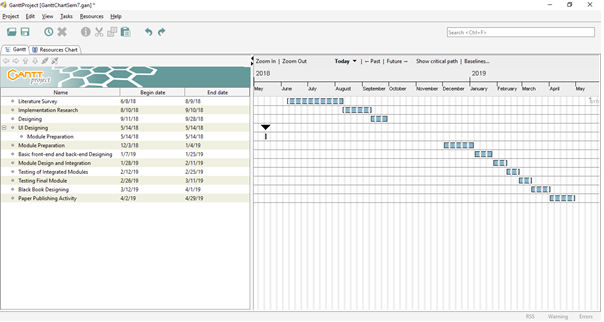
\includegraphics{gantt.png}}
	\caption{Project Time-line}
	\label{fig:gantt}
\end{figure}
\chapter{Software Requirements Specification}
\section{Introduction}
\subsection{Product Overview}
"Speech to 3D Scene Generation" is a software that is developed to provide a near run-time digital/graphical output to the literal spoken words of the user. It goes through various stages before providing the final output. First, the speech is converted to text, then the text is passed to the interpretation protocol, and finally the interpreted text is used to render the output.\linebreak
	The best part of "Speech to 3D Scene Generation" is that it is meant to be used by any person who can speak. It is targeted to be used at various industries like education, creative, etc. as well as corporates. It will run on Windows Desktop Applications. \linebreak
	In general, the software will require APIs and coding platforms that will allow us to convert text to speech and then using speech to render the images.
\section{Specific Requirements}
\subsection{External Interface Requirements}
\textbf{User Interfaces}
\paragraph{} The user interface requirements for “title” is are very general because it is a Desktop application. The PC at the user end should have only the basic screen layouts with no requirements for latest OS. However, it may not be compatible for very earlier versions of Windows OS.\linebreak
	The user should be able to easily navigate to the part where it enables the speaker and the software should immediately start recording, converting and rendering. It is essential that it is simply a one-step process for the user and then it should all be a completely automatic process.\\
	\newline
\textbf{Hardware Interfaces}
\paragraph{} There isn’t much hardware interfaces required since it is a completely software-oriented product. The only requirement is for it to work on any type of PC (Laptop, Computer) which match the basic OS and version requirements.\\
\newline
\textbf{Software Interfaces}
\paragraph{}Softwares Required:
\begin{itemize}
  \item Google Speech-to-Text API (Integrated Library)
  \item SpaCy Version 2.0.13
  \item 3D Warehouse/LFD Laboratory
\end{itemize}
\subsection{Software Product Features}"Speech to 3D Scene Generation" will provide following features:-\newline
\textbf{Functional Requirements}
\begin{enumerate}
  \item Input Data requirements: :
\begin{itemize}
\item Speech Input.
\item JSON as an input data to Database and Rendering.
\end{itemize}
\item Operational requirements
\begin{itemize}
\item Conversion of speech to text.
\item POS tagging.
\item Parse tree generation.
\item Information gathering and rendering.
\end{itemize}
\end{enumerate}
\textbf{Non-functional Requirements}
\begin{enumerate}
  \item Performance: 75\% conversion accuracy. Worst case 15s generation. Best case 3s.
 \item Data Integrity: Data and modules to be kept abstract.
 \item Usability: Smooth screen-to-screen movement.

\end{enumerate}
\subsection{Software System Attributes}
\textbf{Reliability}
\begin{itemize}
  \item Mean Time To Failure (MTTF) is Twenty Seconds.
  \item Expected optimal time for rendering and displaying is Seven Seconds.
  \item Speech-to-Text 75\% accuracy.
\end{itemize}

\textbf{Availability}
\begin{itemize}
  \item Failure at any point of the process will lead to complete termination and the user will have to start and perform the process all over again.
\end{itemize}

\textbf{Security}
\begin{itemize}
  \item Since it is a Desktop application, the basic security measures taken by the user are sufficient with no additional requirements except for basic login credentials.
  \item Data/image/graph rendering is over the internet therefore simple internet security is more than enough.
\end{itemize}

\textbf{Portability}
\begin{itemize}
  \item Entire software is mainly Python-oriented.
  \item No need of external compiler because of integrated environment.
  \item Most commonly used OS (Windows) is all that is required with no additional features.
\end{itemize}

\textbf{Performance}
\begin{itemize}
  \item As mentioned, minimum 75\% accuracy for Google speech-to-text API. Minimum latency for rendering.
  \item Users are expected to provide clear speech inputs, avoiding grammatical errors.
  \item Users are expected to be in a relatively quiet environment so as to ease the processing of the API.
  \item Data storage integrated using cloud therefore not much physical storage required.
\end{itemize}

\subsection{Database Requirements}
\begin{itemize}
\item No database required except for Google 3D Warehouse/LFD Laboratory.
\end{itemize}
\chapter{Software Design Description}
\section{Introduction}
\paragraph{}The design phase is aimed at the creative and adequate design of the project. The design phase focuses on the design and structure of the app, its relations with the main database as well as working of the app on a stand-alone basis. This phase also includes the information of various modules and diagrams which are used as figurative representation of the design and app working.
\subsection{Design Overview}\paragraph{}The architectural design is to be implemented in a manner which clearly conveys the flow of data and input/output streams. Each module is placed with respect to the actions performed by that module, the outcomes of the module, and the other modules affecting with those outcomes, so as to maintain the efficiency of the software with minimum time consumption.
It can also be observed that some parts of the design have sub-modules as well such as geometric knowledge, linguistic knowledge, etc. which are going to be used by the parent module only, therefore in such cases it is made sure that these sub-modules do not interact and interrupt/interfere with the other parts of the design. During the software design phase, the implementation team will recommend how the system will be configured to support the industry needs.
\newpage
\subsection{Requirements Traceability Matrix}
  \begin{center}
\begin{table}[h!]
\caption{Requirements Traceability Matrix}
  \centering
  \begin{tabular}{|p{3cm}| p{1.5cm} | p{1.5cm} | p{1.5cm}|}
\hline
    Functional requirements. & User.& User Accounts. & Server.\\
    \hline
    
    Login. &X&X&\\
 \hline
    Speech Input. &X&X&X\\
 \hline
    Database Manipulation.&&X&\\
 \hline
    Data Storage.&X&&X\\
 \hline

  \end{tabular}
\end{table}
\end{center}

\section{System Architectural Design}
\subsection{Chosen System Architecture} 
\textbf{Tier-1 Architecture}
\paragraph{}Figure 5.1 includes all the modules and interfaces involved in the project. The foremost step is to provide the speech input. This speech input will be received by the speech to text API, which will convert the provided speech to text.
\linebreak Next step is interpretation; this is where the converted text is being processed by SpaCy library used in Python environment. The term interpretation means that the text will be divided into multiple parts of speech identified by the library. As you can see, the library will make use of linguistic and word knowledge to precisely identify which word from the word knowledge (dictionary) fits into which category of the English language.
\linebreak One the text is vividly classified, the database (3D Warehouse) comes into action. Note that the hierarchy created by SpaCy is the most important part. The database will use the hierarchy to identify the order in which the scene is to be generated and more importantly, the relation between the objects of the scene, along with the attributes of each object and the scene as a whole. It will require extensive geometric knowledge to place the objects exactly where required and also for mathematical purposes for forming a grid. Once all this is done, the scene will simply be rendered to the designed UI.
\newpage
\begin{figure}[htbp]
	\centering
		\frame{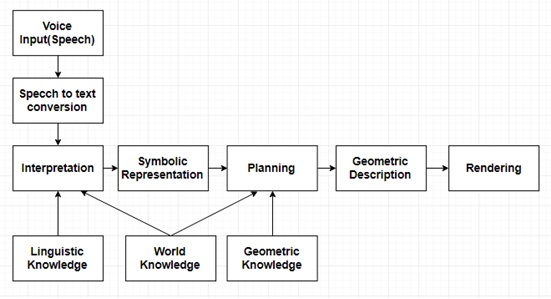
\includegraphics[width=350px,height=300px]{architecture.jpg}}
	\caption{Architecture design}
	\label{fig:architecture}
\end{figure}

\newpage

\subsection{System Interface Description}
\paragraph{}
The software is a desktop application and thus, will work on Windows OS. The user will simply need to install the software and it will be ready to use. All the libraries and database files will run in the background, potentially using cloud, therefore the user will only need to download and install the installer and main file.\\
The APIs and libraries used by the software are Speech to Text API, SpaCy library and 3D Warehouse database/dataset. All the components are back end products and therefore beyond users’ control and reach. The knowledge/information sets are also integrated with the APIs and libraries hence not concerning the user.
\section{User Interface Design}

\subsection{Screen Images}
\begin{figure}[htbp]
	\centering
		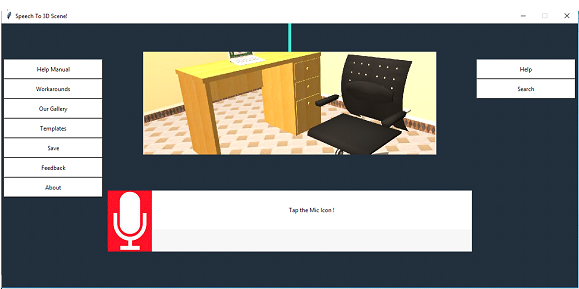
\includegraphics{ui2.png}
	\caption{User Interface}
	\label{fig:ui2}
\end{figure}
\newpage

\section{Design Document}
\subsection{Level 0 DFD}
\begin{figure}[htbp]
	\centering
		\frame{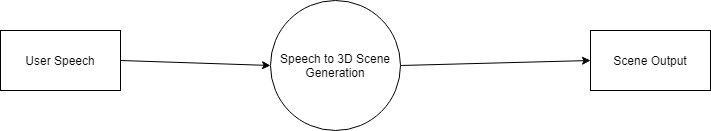
\includegraphics[width=390px]{dfd0.png}}
	\caption{DFD Level 0}
	\label{fig:dfd0}
\end{figure}

\subsection{Level 1 DFD}
\begin{figure}[htbp]
	\centering
		\frame{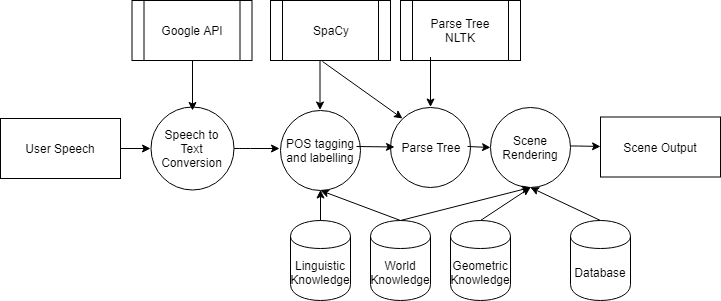
\includegraphics[width=380px,height=200px]{dfd1.png}}
	\caption{DFD Level 1}
	\label{fig:dfd1}
\end{figure}

\newpage

\subsection{Use Case Diagram}
\begin{figure}[htbp]
	\centering
		\frame{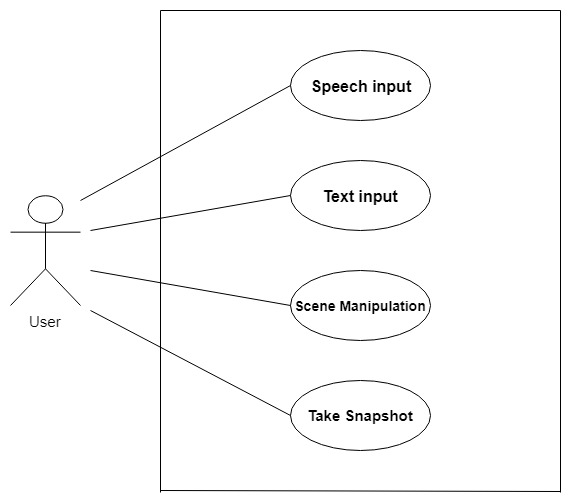
\includegraphics[width=390px]{Use_Case_Diagram.jpg}}
	\caption{Use Case Diagram}
	\label{fig:Use_Case_Diagram}
\end{figure}

\newpage

\subsection{Class Diagram}
\begin{figure}[htbp]
	\centering
		\frame{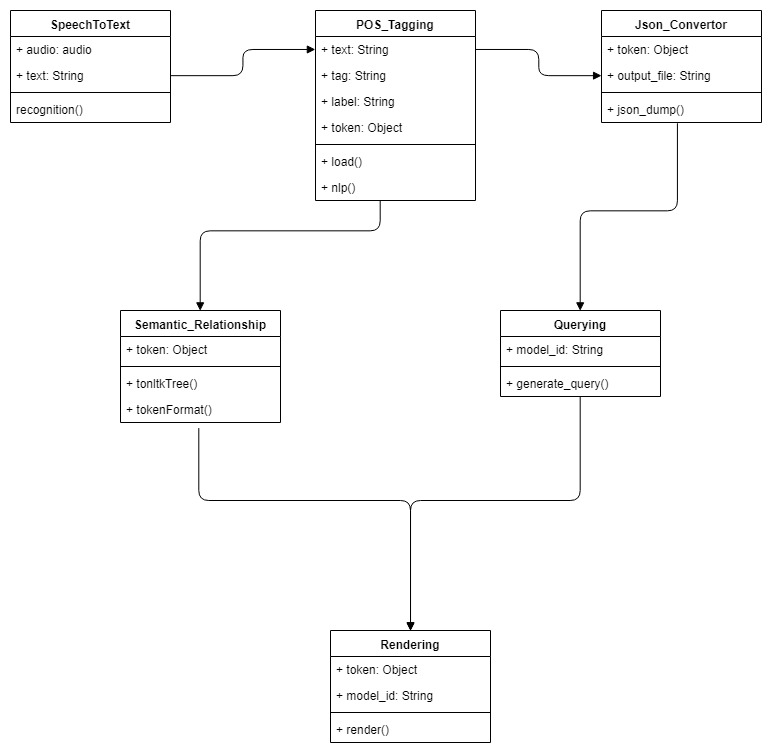
\includegraphics[width=390px]{Class_Diagram.jpg}}
	\caption{Class Diagram}
	\label{fig:Class_Diagram}
\end{figure}

\newpage

\subsection{Activity Diagram}
\begin{figure}[htbp]
	\centering
		\frame{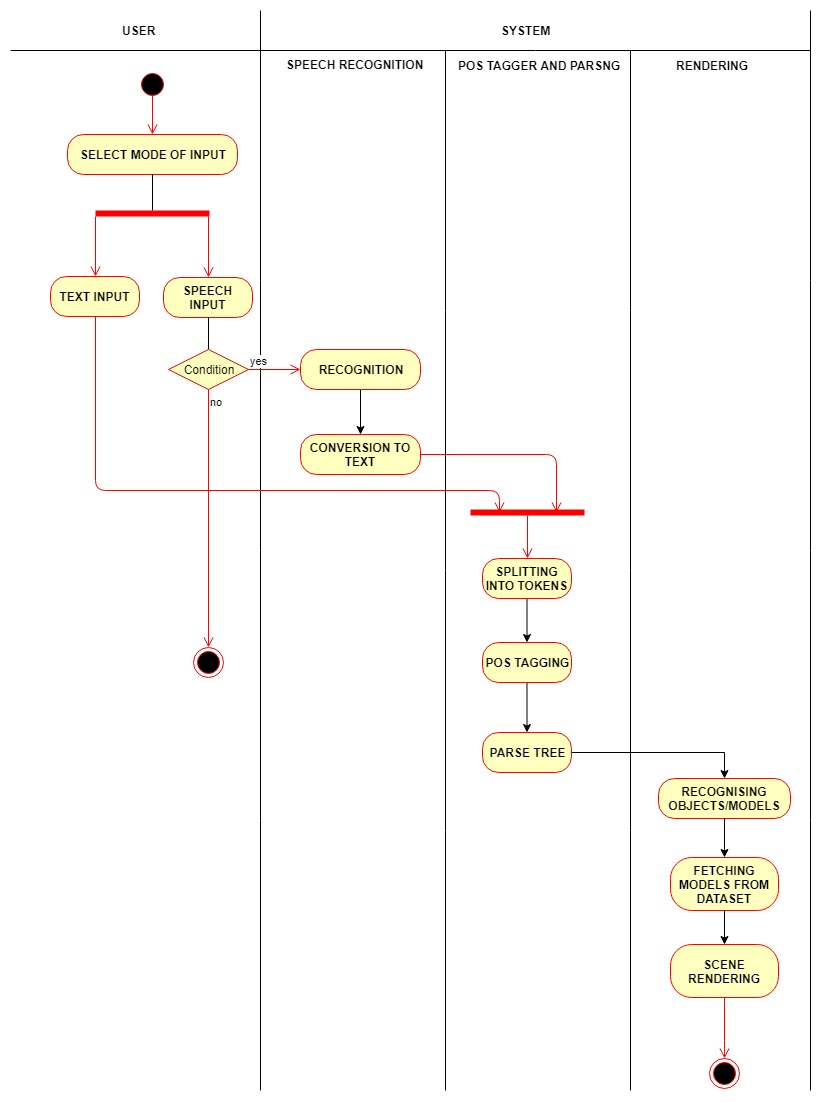
\includegraphics[width=390px,height=430px]{Activity_Diagram.jpg}}
	\caption{Activity Diagram}
	\label{fig:Activity_Diagram}
\end{figure}
\chapter{Software Test Document}
\section{Introduction}

\subsection{System Overview}
\paragraph{}Speech to 3d Scene generator is a software application developed to provide a near real time 3D scene. It goes through various stages before providing the output. Speech input in converted into text, then the text is processed using natural language processing and broken down into low level parts of speech tags.
	A parse tree generating a semantic relationship is generated which will further be used to generate and fire queries dynamically to a 3d model database. The 3d models extracted from the model database will be rendered on a model viewer and positioned with respect to other models in that scene. Any queries fired further will manipulate the existing scene in near real time.
\newpage
\subsection{Test Approach} 
\begin{table}[h!]
\caption{Test Approach}
  \centering
  \begin{tabular}{|p{3.5cm}|p{10cm}|}
\hline
   TEST& DESCRIPTION.\\
    \hline
    Unit Testing &The purpose is to validate that each unit of the software performs as designed. Units like speech to text, parts of speech tagging, semantic relations and database handlers are tested.\\
    \hline
    Integration Testing &The purpose of this testing is to expose faults in the interaction between integrated units. Above mentioned modules are tested to remove faults.\\

\hline
    Functional Testing  &Includes testing of all database handlers. Input from the user is validated against various test cases.\\
\hline
    Usability Testing &The application will be checked for user friendliness and comfort. Each user function is tested which includes test for navigation and buttons, content checking.\\
 \hline

  \end{tabular}
\end{table}

\subsection{ Features to be tested }
\begin{enumerate}
\item \textbf{Speech to text Conversion}
\item \textbf{Scene Generation}
\item \textbf{Scene Manipulation }
\end{enumerate}

\subsection{Features not to be tested}
\begin{enumerate}
\item \textbf{Parts of Speech Tagging.}
\item \textbf{Label are not to be tested.}
\end{enumerate}

\subsection{Testing Tools and Environment}
\paragraph{}Testing of the software application will require 15-25 days. Manual as well automated testing approaches will be applied.\\
\textbf{1. AutoIT : }AutoIT is a Stand Alone (doesn’t require any configuration) and small footprint tool, that simulates mouse and keyboard clicks . It activates the binary files of the tested app using a Reflection.\linebreak The AutoIT comes with dedicated IDE, and is compatible with recordings and coding in its own scripting language (very similar to BASIC syntax). \\

\textbf{2. TestStack.White : }White is a library for automation of desktop apps. It started as a small open source project and then became a part of TestStack which consists of a variety of open source code projects for automated and manual testing.\linebreak White supports a variety of automation technologies: Silverlight, WPF, WinForms, Win32 and SWT in Java. It’s possible to write White tests in any language supported by .NET.\\

\textbf{3. Pywinauto : }The PyWinAuto is a Python library that provides a collection of functions that make operations on Windows (controls and windows dialogs). The library presents a wide set of operations, is clear and user friendly.
\newpage
\section{Test Cases}
 \begin{table}[h!]
 \caption{Test Cases}
  \centering

  \begin{tabular}{|p{2.5cm}|p{4.5cm}|p{2cm}|p{4.5cm}|}
\hline
    Test Case&Purpose& Input&Expected output\\
    \hline
   Speech to text conversion&Whether the input speech converted into the text is valid for the further processing or not. To check how accurate, the speech is converted is converted into text.&Voice Input&The text is valid if the text converted is same as the speech input given by the user. If it is then text is further processed else user can rerecord the input.\\
    \hline
   Tagging and Labelling&To check whether the parts of speech tagging and labelling of the text is done meaningfully or not.&Text Converted using Speech to text Recognition.&JSON or XML file which will contain proper parts of speech tagging and labelling of the text.\\
 \hline
  Rendered Models& To check whether the rendered models from data warehouse are perfectly suitable with the input provided in first stage.&No input from the user, the converted text is processed further.&Actual model of specific objects specified by the user are correctly rendered else final output will be incorrect, Models should not overlap.\\
 \hline
   Positions of the object (models)&To check whether the models rendered and displayed on the output screen are at proper coordinates as user wants.&No specific input, Text is processed&Objects are at proper position as mentioned by the user into the speech input.\\

 \hline

  \end{tabular}
\end{table}

\renewcommand{\bibname}{References}
\bibliographystyle{unsrt}
\bibliographystyle{plainnat}
\renewcommand{\bibliography}{\References}
\addcontentsline{toc}{chapter}{References}
%%\bibliography{author}
\begin{thebibliography}{9}
		\bibitem{wordsEye} 
		Bob Coyne and Richard Sproat. “WordsEye: an automatic text-to-scene conversion system”. In Proceedings of the 28th annual conference on Computer graphics and interactive techniques, 2001.
		\bibitem{nlp}
		Lee M Seversky and Lijun Yin.“Real-time automatic 3D scene generation from natural language voice and text descriptions”. In Proceedings of the14th annual ACM international conference on Multimedia ,2006.
		\bibitem{AI}
		R. Johansson, A. Berglund, M. Danielsson, "Artificial Intelligence" The Nineteenth International Joint Conference , pages 1073–1078, 2005.
		
\end{thebibliography}
%% refer q31.tex

\newpage
\begin{center}
\textbf{\begin{LARGE}Acknowledgement\end{LARGE}}
\end{center}

\vspace{1.5cm}
I take this opportunity to express my profound gratitude and deep regards to my guide Prof. Sagar Korde for his exemplary guidance, monitoring and constant encouragement throughout the course of this project.\\
 I also take this opportunity to express a deep sense of gratitude to Head of the department, Prof. Sujata Pathak for her cordial support, valuable information and guidance, which helped me in completing this task through various stages.\\
 I am obliged to staff members of K. J. Somaiya College of Engineering, for the valuable information provided by them in their respective fields. I am grateful for their cooperation during the period of our assignment.




\vspace{1in}\\


\begin{flushleft}
Date:
\end{flushleft}

\begin{flushright}
\begin{large}Manthan Turakhia\\Umang Nandu\\Prayesh Shah\\Siddharth Sharma\end{large}
\end{flushright}





\end{document}